\begin{frame}[fragile,label=2BmispredEx]{exercise}
\begin{itemize}
\item use 2-bit predictor on this loop
    \begin{itemize}
    \item executed in outer loop (not shown) many, many times
    \end{itemize}
\item what is the conditional branch misprediction rate?
\end{itemize}
\begin{lstlisting}[language=C,style=small]
int i = 0;
while (true) {
  if (i % 3 == 0) goto next;
  ...
next:
  i += 1;
  if (i == 50) break;
}
\end{lstlisting}
\end{frame}

\ifdefined\exCode\else\newsavebox\exCode\fi
\begin{lrbox}{\exCode}
\begin{lstlisting}[language=C,style=smaller]
int i = 0;
while (true) {
  if (i % 3 == 0) goto next;
  ...
next:
  i += 1;
  if (i == 50) break;
}
\end{lstlisting}
\end{lrbox}

\begin{frame}<0>[label=2BmispredExSoln]{exercise soln (1)}
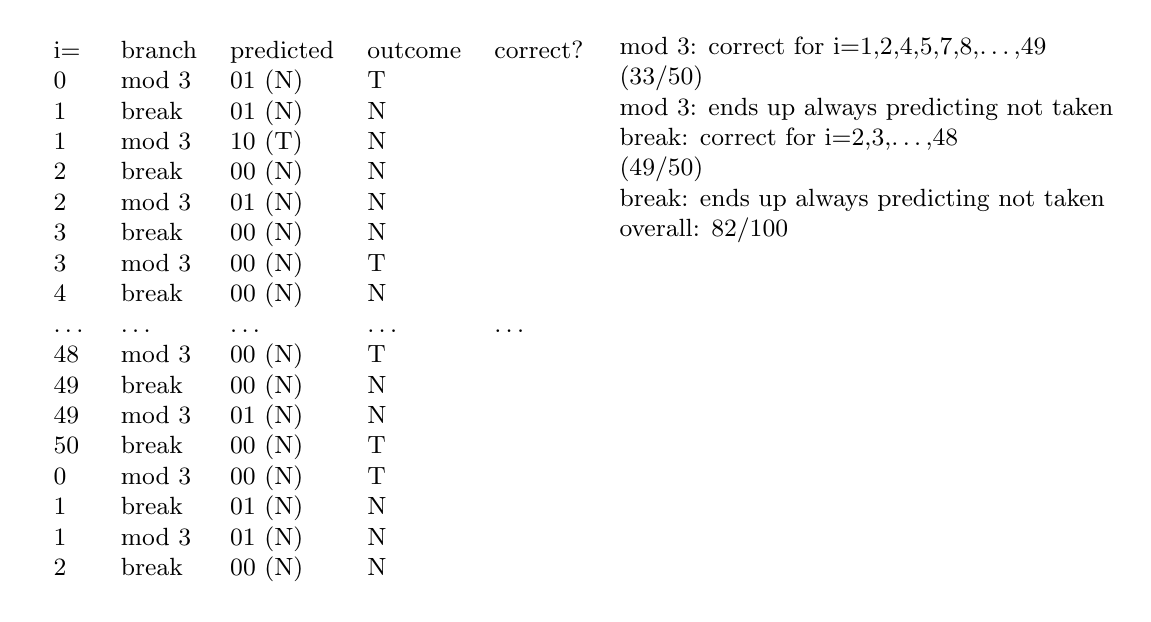
\begin{tikzpicture}
\node[font=\small] (table) {
\begin{tabular}{lllll}
i= & branch & predicted & outcome & correct? \\
0 & mod 3 & 01 (N) & T & \\
1 & break & 01 (N) & N & \checkmark \\
1 & mod 3 & 10 (T) & N & \\
2 & break & 00 (N) & N & \checkmark \\
2 & mod 3 & 01 (N) & N & \checkmark \\
3 & break & 00 (N) & N & \checkmark \\
3 & mod 3 & 00 (N) & T & \\
4 & break & 00 (N) & N & \checkmark \\
\ldots & \ldots & \ldots & \ldots  & \ldots \\
48 & mod 3 & 00 (N)  & T & \\
49 & break & 00 (N) & N & \checkmark \\
49 & mod 3 & 01 (N) & N & \checkmark \\
50 & break & 00 (N) & T & \\
0 & mod 3 & 00 (N) & T &\\
1 & break & 01 (N) & N & \checkmark \\
1 & mod 3 & 01 (N) & N & \checkmark \\
2 & break & 00 (N) & N & \checkmark \\
\end{tabular}
};
\node[anchor=north west,align=left,font=\small](conclude) at (table.north east) {
mod 3: correct for i=1,2,4,5,7,8,\ldots,49 \\
(33/50) \\
mod 3: ends up always predicting not taken \\
break: correct for i=2,3,\ldots,48 \\
(49/50) \\
break: ends up always predicting not taken \\
overall: 82/100
};
\node[anchor=north west] at (conclude.south west) {
\usebox{\exCode}
};
\end{tikzpicture}
\end{frame}

\iftoggle{heldback}{}{\againframe<1->{2BmispredExSoln}}
